% !TeX spellcheck = fr_FR
\documentclass[a4paper,11pt,oneside,roman]{article}
    \usepackage[utf8]{inputenc}
    \usepackage[T1]{fontenc}
    \usepackage[top=2cm, left=2cm, right=2cm, bottom=2cm]{geometry}
    \usepackage[francais]{babel}
    \usepackage[hidelinks=true]{hyperref}
    \usepackage{listings}
    \usepackage{color}
    \usepackage{amsmath}
    \usepackage{graphicx}
    \usepackage{amssymb}
    \usepackage{natbib}
    \usepackage{float}
    \usepackage{hyperref}
    \usepackage{advdate}
    
    \floatplacement{figure}{H}
    
    \definecolor{dkgreen}{rgb}{0,0.6,0}
    \definecolor{gray}{rgb}{0.5,0.5,0.5}
    \definecolor{mauve}{rgb}{0.58,0,0.82}
    
    \linespread{1.3} %space between lines
    \setlength{\parskip}{1em}  %space between paragraphs
    
    \begin{document}
    
    \begin{titlepage}
    
        \newcommand{\HRule}{\rule{\linewidth}{0.5mm}} % Defines a new command for the horizontal lines, change thickness here
        
        \center % Center everything on the page
         
        %----------------------------------------------------------------------------------------
        %	HEADING SECTIONS
        %----------------------------------------------------------------------------------------
        
        \textsc{\LARGE Université de Technologie de Compiègne}\\[0.5cm] % Name of your university/college
        \textsc{\Large Génie informatique}\\[1.5cm] % Name of your university/college
        
        %----------------------------------------------------------------------------------------
        %	TITLE SECTION
        %----------------------------------------------------------------------------------------
        
        \HRule \\[0.4cm]
        { \huge \bfseries Entrainement d'un réseau de neurones et rétropropagation dans le cadre d'un problème de classification.}\\[0.4cm] % Title of your document
        \HRule \\[1.5cm]
         
        %----------------------------------------------------------------------------------------
        %	AUTHOR SECTION
        %----------------------------------------------------------------------------------------
        
        % If you don't want a supervisor, uncomment the two lines below and remove the section above
        \Large \emph{Authors:}\\
        Nacim \textsc{Khalis} et Antoine \textsc{Collas}\\[3cm] % Your name
        
        %----------------------------------------------------------------------------------------
        %	DATE SECTION
        %----------------------------------------------------------------------------------------
        
        {\large \AdvanceDate[-4]\today}\\[4cm] % Date, change the \today to a set date if you want to be precise
        
        %----------------------------------------------------------------------------------------
        %	LOGO SECTION
        %----------------------------------------------------------------------------------------
        
        
\includegraphics[width=0.5\textwidth]{imgs/logo_UTC_SU.jpg}\\[1cm] % Include a department/university logo - this will require the graphicx package
        
        %----------------------------------------------------------------------------------------
        
        \vfill % Fill the rest of the page with whitespace
        
    \end{titlepage}
    
    % \tableofcontents
    
    \pagebreak
        
    \section{Réseau de neurones: perceptron multicouche}
    
    L'objectif est de programmer un perceptron multicouche afin de classer un ensemble de bouteilles de vins en 3 ensembles.

    L'architecture de notre perceptron multicouche est la suivante:
    \begin{figure}
        \centering
        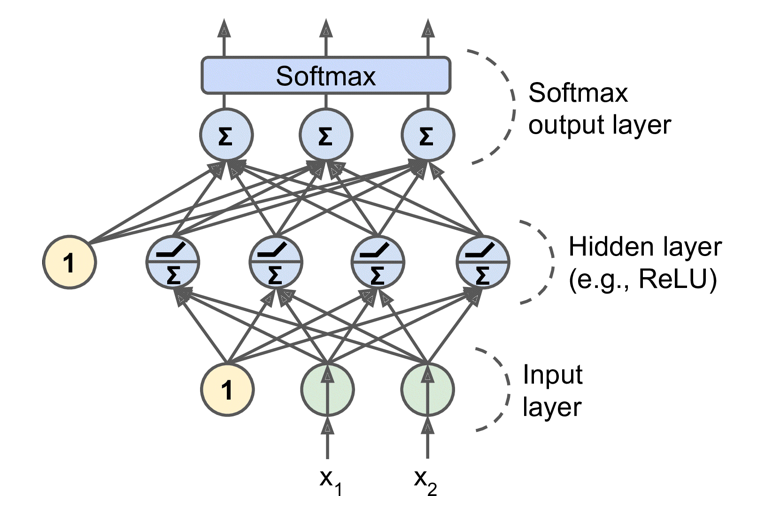
\includegraphics[width=0.5\textwidth]{imgs/perceptron.png}
        \caption{Perceptron multi-couches tiré de 'Hands-On Machine Learning with Scikit-Learn and TensorFlow' de Aurélien Géron.}
        \label{fig_perceptron}
    \end{figure}

    \section{Entrainement d'un réseau de neurones de classification}
    \subsection{Notation}
    $m$ est le nombre d'éléments dans notre ensemble d'entrainement.

    $K$ est le nombre de classes (et donc de sorties de notre réseau de neurones).

    $n_{in}$ est le nombre de neurones de la couche d'entrée (sans le biais). Donc $n_{in}$ correspond à la dimension de nos données d'entrée.
    
    $n_{hidden}$ est le nombre de neurones de la couche cachée (sans le biais).
    
    $n_{out}$ est le nombre de neurones de la couche de sortie. Donc $n_{out}$ correspond au nombre de classes de notre problème.
    
    $b_i^{(l)}$ est le biais de la couche $l$ allant vers le ième neurone de la couche $l+1$.

    $w_{ij}^{(l)}$ est le poids entre le neurone $i$ de la couche $l$ et le neurone $j$ de la couche $l+1$.
    
    $x_{i}^{(l)}$ est la sortie du neurone $i$ de la couche $l$. Donc $x_{i}^{(2)} = relu(\sum\limits_{k=1}^{n_{in}} w_{ki}^{(1)}x_{k}^{(1)} + b_i^{(1)})$
    
    $relu(x) = max(0,x)$ est la fonction d'activation de la couche cachée.

    $softmax(x)_j = \frac{e^{x_j}}{\sum\limits_{k=1}^n e^{x_k}}$ est la fonction de sortie permettant d'obtenir la probabilité pour chaque classe.

    $E = -\frac{1}{m} \sum\limits_{i=1}^m\sum\limits_{k=1}^K (y_{k}^{(i)} \times log(\hat{p}_{k}^{(i)}))$ est l'erreur appelée entropie croisée.
    $y_{k}^{(i)}$ vaut 1 si le ième élément de l'échantillon appartient à la classe $k$, 0 sinon. $\hat{p}_{k}^{(i)}$ est la kème sortie du perceptron pour le ième élément de l'échantillon.

    \subsection{Calcul des dérivées partielles de la fonction de coût}

    L'apprentissage d'un réseau de neurones est executé à l'aide d'une descente de gradient sur la fonction de coût. Les paramètres de notre réseau sont les poids $w_{ij}^{(l)}$ et les biais $b_j^{(l)}$.
    Nous cherchons donc à calculer les dérivées partielles de la fonction de coût par rapport à ces différents paramètres. Nous commençons par montrer comment calculer $\frac{\partial E}{\partial w_{ij}^{(2)}}$ $\forall (i,j) \in \{1, ..., n_{hidden}\} \times \{1, ..., n_{out}\}.$

    Pour un lot de données entré dans le réseau nous avons les équations suivantes en partant de l'erreur:
    
    \begin{equation}
        E = -\frac{1}{m} \sum\limits_{p=1}^m\sum\limits_{k=1}^K (y_{k}^{(p)} \times log(\hat{p}_{k}^{(p)}))
    \end{equation}
avec 
    \begin{equation}
        \hat{p}_{k}^{(p)} = softmax(x^{(p,3)})_k
    \end{equation}
    où $x^{(p,3)}$ est la sortie de la dernière couche avant le softmax pour la pème donnée d'entrainement.

    \begin{equation}
        \frac{\partial E}{\partial w_{ij}^{(2)}} = -\frac{1}{m} \sum\limits_{p=1}^{m} \sum\limits_{k=1}^{n_{out}} y_k^{(p)} \frac{\partial log(\hat{p}_{k}^{(p)})}{\partial w_{ij}^{(2)}}
    \end{equation}

    Règle de la chaine:
    si $y = f(u)$ et $u=g(x)=(g_1(x), ..., g_m(x))$ alors $\frac{\partial y}{\partial x_i} = \sum\limits_{l=1}^{m} \frac{\partial y}{\partial u_l} \frac{\partial u_l}{\partial x_i}$
    
    Donc en appliquant la règle de la chaine:
    
    \begin{equation}
        \frac{\partial log(\hat{p}_{k}^{(p)})}{\partial w_{ij}^{(2)}} = \sum\limits_{q=1}^{n_{out}} \frac{\partial log(\hat{p}_{k}^{(p)})}{\partial (x^{(p,3)})_{q}} \frac{\partial (x^{(p,3)})_{q}}{\partial w_{ij}^{(2)}}
    \end{equation}
    
    or si $q \ne j$
    \begin{equation}
       \frac{\partial (x^{(p,3)})_{q}}{\partial w_{ij}^{(2)}} = 0
    \end{equation}
    
    donc
    \begin{equation}
        \frac{\partial log(\hat{p}_{k}^{(p)})}{\partial w_{ij}^{(2)}} = \frac{\partial log(\hat{p}_{k}^{(p)})}{\partial (x^{(p,3)})_{j}} \frac{\partial (x^{(p,3)})_{j}}{\partial w_{ij}^{(2)}}
    \end{equation}

    \begin{equation}
        log(\hat{p}_{k}^{(p)}) = \frac{ln(\hat{p}_{k}^{(p)})}{ln(10)} = \frac{(x^{(p,3)})_k - ln(\sum\limits_{q=1}^{n_{out}} e^{(x^{(p,3)})_q})} {ln(10)}
    \end{equation}

    Si $k \ne j$
    \begin{equation}
        \frac{\partial log(\hat{p}_{k}^{(p)})}{\partial (x^{(p,3)})_{j}} = -\frac{1}{ln(10)} \frac{e^{(x^{(p,3)})_j}}{\sum\limits_{q=1}^{n_{out}} e^{(x^{(p,3)})_q}} = -\frac{softmax(x^{(p,3)})_j}{ln(10)}
    \end{equation}

    Sinon (dans le cas où $k = j$):
    \begin{equation}
        \frac{\partial log(\hat{p}_{k}^{(p)})}{\partial (x^{(p,3)})_{j}} = \frac{1}{ln(10)} \bigg[ 1 - softmax(x^{(p,3)})_j \bigg]
    \end{equation}

    Donc $\forall k$:
    \begin{equation}
        \frac{\partial log(\hat{p}_{k}^{(p)})}{\partial (x^{(p,3)})_{j}} = \frac{1}{ln(10)} \bigg[ \delta_{kj} - softmax(x^{(p,3)})_j \bigg]
        \label{log_x3}
    \end{equation}
    
    où $ \delta_{kj} = 1$ si $k = j$, $0$ sinon.
    
    De plus,
    \begin{equation}
        (x^{(p,3)})_{j} = \sum\limits_{i=1}^{n_{hidden}} w_{ij}^{(2)}(x^{(p,2)})_i + b_j^{(2)}
    \end{equation}

    Donc,
    \begin{equation}
        \frac{\partial (x^{(p,3)})_{q}}{\partial w^{(2)}_{ij}} = (x^{(p,2)})_i
    \end{equation}

    \begin{equation}
        \frac{\partial log(\hat{p}_{k}^{(p)})}{\partial w^{(2)}_{ij}} = \frac{1}{ln(10)} \bigg[ \delta_{kj} - softmax(x^{(p,3)})_j \bigg] (x^{(p,2)})_{i}
    \end{equation}

    Ce qui donne finalement:
    \begin{equation}
        \frac{\partial E}{\partial w_{ij}^{(2)}} = -\frac{1}{m \times ln(10)} \sum\limits_{p=1}^{m} \sum\limits_{k=1}^{n_{out}} y_k^{(p)} \bigg[ \delta_{kj} - softmax(x^{(p,3)})_j \bigg] (x^{(p,2)})_{i}
    \end{equation}

    Cette formule peut être interprétée de la manière suivante:
    \begin{itemize}
        \item Si la classe à prédire pour la $p^{eme}$ donnée entrée dans le réseau est $j$ alors le poids $w_{ij}^{(2)}$ est augmenté en fonction de la performance de la prédiction et de $(x^{(p,2)})_{i}$.
        Si la prédiction est déjà très bonne, $w_{ij}^{(2)}$ n'est est que légèrement augmenté sinon il est formetement augmenté pour augmenter la probabilité sortante du réseau.
        \item Si la classe à prédire est $k \ne j$ alors il y une diminution du poids en fonction de la probabilité sortante et de $(x^{(p,2)})_{i}$. Si la probabilité sortante est faible, le poids n'est que légèrement diminué. Si elle est élevée (alors qu'elle devrait être faible), le poids est fortement diminué.
    \end{itemize}

    Nous appliquons le même procédé pour calculer $\frac{\partial E}{\partial w_{ij}^{(1)}}$

    \begin{equation}
        \frac{\partial E}{\partial w_{ij}^{(1)}} = -\frac{1}{m} \sum\limits_{p=1}^{m} \sum\limits_{k=1}^{n_{out}} y_k^{(p)} \frac{\partial log(\hat{p}_{k}^{(p)})}{\partial w_{ij}^{(1)}}
        \label{E_wij1}
    \end{equation}

    \begin{equation}
        \frac{\partial log(\hat{p}_{k}^{(p)})}{\partial w_{ij}^{(1)}} = \frac{\partial log(\hat{p}_{k}^{(p)})}{\partial (x^{(p,2)})_j} \frac{\partial (x^{(p,2)})_j}{\partial w_{ij}^{(1)}}
        \label{log_wij}
    \end{equation}

    \begin{equation}
        \frac{\partial log(\hat{p}_{k}^{(p)})}{\partial (x^{(p,2)})_j} = \sum\limits_{q=1}^{n_{out}} \frac{\partial log(\hat{p}_{k}^{(p)})}{\partial (x^{(p,3)})_q} \frac{\partial (x^{(p,3)})_q}{\partial (x^{(p,2)})_j}
        \label{log_x2}
    \end{equation}
    
    \begin{equation}
        \frac{\partial (x^{(p,3)})_k}{\partial (x^{(p,2)})_j} = w_{jk}^{(2)}
        \label{x3_x2}
    \end{equation}
    
    D'après les équations \eqref{log_x3}, \eqref{log_x2}, \eqref{x3_x2}:
    \begin{equation}
        \frac{\partial log(\hat{p}_{k}^{(p)})}{\partial (x^{(p,2)})_j} = \frac{1}{ln(10)} \sum\limits_{q=1}^{n_{out}} \bigg[ \delta_{kq} - softmax(x^{(p,3)})_q \bigg] w_{jk}^{(2)}
        \label{log_x2_final}
    \end{equation}
    
    \begin{equation}
        (x^{(p,2)})_{j} = relu\bigg[\sum\limits_{k=1}^{n_{in}} w_{kj}^{(1)}(x^{(p,1)})_{k} + b_j^{(1)}\bigg]
    \end{equation}
    
    Si $\sum\limits_{k=1}^{n_{in}} w_{kj}^{(1)}(x^{(p,1)})_{k} + b_j^{(1)} > 0$:
    \begin{equation}
        \frac{\partial (x^{(p,2)})_j}{\partial w_{ij}^{(1)}} = \frac{\partial relu\bigg[\sum\limits_{k=1}^{n_{in}} w_{kj}^{(1)}(x^{(p,1)})_{k} + b_j^{(1)}\bigg]}{\partial w_{ij}^{(1)}} = \frac{\partial \bigg[\sum\limits_{k=1}^{n_{in}} w_{kj}^{(1)}(x^{(p,1)})_{k} + b_j^{(1)}\bigg]}{\partial w_{ij}^{(1)}} = (x^{(p,1)})_i
    \end{equation}
    
    Si $\sum\limits_{k=1}^{n_{in}} w_{kj}^{(1)}(x^{(p,1)})_{k} + b_j^{(1)} < 0$:
    \begin{equation}
        \frac{\partial (x^{(p,2)})_j}{\partial w_{ij}^{(1)}} = \frac{\partial relu\bigg[\sum\limits_{k=1}^{n_{in}} w_{kj}^{(1)}(x^{(p,1)})_{k} + b_j^{(1)}\bigg]}{\partial w_{ij}^{(1)}} = 0
    \end{equation}
    
    Donc:
    \begin{equation}
        \frac{\partial (x^{(p,2)})_j}{\partial w_{ij}^{(1)}} = H\bigg[\sum\limits_{k=1}^{n_{in}} w_{kj}^{(1)}(x^{(p,1)})_{k} + b_j^{(1)}\bigg](x^{(p,1)})_i
        \label{x2_wij}
    \end{equation}
    où $H(x) = 1$ si $x>0$, et $0$ si $x<0$.

    %16,19,23
    D'après les équations \eqref{log_wij}, \eqref{log_x2_final}, \eqref{x2_wij}:
    \begin{equation}
        \frac{\partial log(\hat{p}_{k}^{(p)})}{\partial w_{ij}^{(1)}} = \frac{1}{ln(10)} H\bigg[\sum\limits_{q=1}^{n_{in}} w_{qj}^{(1)}(x^{(p,1)})_{q} + b_j^{(1)}\bigg](x^{(p,1)})_i \sum\limits_{q=1}^{n_{out}} \bigg[\big[ \delta_{kq} - softmax(x^{(p,3)})_q \big] w_{jq}^{(2)} \bigg] 
        \label{log_wij_final}
    \end{equation}

    D'après les équations \eqref{E_wij1} et \eqref{log_wij_final}:
    \begin{equation}
        \frac{\partial E}{\partial w_{ij}^{(1)}} = -\frac{1}{m \times ln(10)}  \sum\limits_{k=1}^{n_{out}} \sum\limits_{p=1}^{m} \Bigg[ y_k^{(p)} \sum\limits_{q=1}^{n_{out}} \bigg[ \big[ \delta_{kq} - softmax(x^{(p,3)})_q \big] w_{jq}^{(2)} \bigg] H\big[\sum\limits_{q=1}^{n_{in}} w_{qj}^{(1)}(x^{(p,1)})_{q} + b_j^{(1)}\big](x^{(p,1)})_i \Bigg]
    \end{equation}

    Autre écriture:

    \begin{equation}
        \frac{\partial E}{\partial w_{ij}^{(1)}} = -\frac{1}{m \times ln(10)} \sum\limits_{p=1}^{m} \Bigg[ H\big[\sum\limits_{q=1}^{n_{in}} w_{qj}^{(1)}(x^{(p,1)})_{q} + b_j^{(1)}\big](x^{(p,1)})_i   \sum\limits_{k=1}^{n_{out}} \bigg[ y_k^{(p)} \sum\limits_{q=1}^{n_{out}} \Big[ \big[ \delta_{kq} - softmax(x^{(p,3)})_q \big] w_{jq}^{(2)} \Big] \bigg] \Bigg]
    \end{equation}

    Interprétation:
    d'après la formule précédente, le changement de $w_{ij}^{(1)}$ est déterminé de la façon suivante:
    \begin{itemize}
        \item nous réunissons tous les éléments d'entrainement par classe (interprétation de la double somme et de $y_k^{(p)}$)
        \item pour chaque élément de la classe nous calculons la responsabilité de $w_{ij}^{(1)}$ dans l'erreur finale: si pour l'élément choisi, la somme pondérée est négative alors le poids n'est pas modifié (pas de responsabilité dans l'erreur, représenté par H dans l'équation)
        \item sinon la modification est proportionnelle à $(x^{(p,1)})_i$ (la variable d'entrée pour le $p^{eme}$ élément d'entrainement) 
        \item la modification est aussi proportionnelle aux erreurs de toutes les sorties (les couches sont totalement connectées ce qui est visible dans $\sum\limits_{q=1}^{n_{out}} \bigg[ \big[ \delta_{kq} - softmax(x^{(p,3)})_q \big] w_{jq}^{(2)} \bigg]$)
    \end{itemize}
    % \begin{equation}
    %     x^{(3)} = (x^{(3)}_1, ..., x^{(3)}_{n_{out}}) = (\sum\limits_{k=1}^{n_{hidden}} w_{k1}^{(2)}x_{k}^{(2)} + b_1^{(2)}, ..., \sum\limits_{k=1}^{n_{hidden}} w_{kn_{out}}^{(2)}x_{k}^{(2)} + b_{n_{out}}^{(2)})
    % \end{equation}

    \section{Rétropropagation}

    Nous avons montré dans la section précédente comment calculer les dérivées partielles de la fonction de coût. Cependant les calculs deviennent rapidement assez complexes et peu efficaces en terme de performances.
    Nous voyons qu'il va être très compliqué d'ajouter des couches cachées supplémentaires à notre réseau.
    Nous allons maintenant détailler l'algorithme de rétropropagation du gradient qui permet de calculer les gradients successivements en appliquant astucieusement la règle de la chaîne.

    Soit $E^p$ l'erreur pour la $p^{eme}$ donnée:
    \begin{equation}
        E^p = - \sum\limits_{k=1}^K (y_{k}^{(p)} \times log(\hat{p}_{k}^{(p)}))
    \end{equation}

    En appliquant la règle de la chaine:
    \begin{equation}
        \begin{aligned}
            \frac{\partial E^p}{\partial w_{ij}^{(1)}} & = \frac{\partial E^p}{\partial (x^{(p,2)})_j} \frac{\partial (x^{(p,2)})_j}{\partial (\sum\limits_{k=1}^{n_{in}} w_{kj}^{(1)}(x^{(p,1)})_{k} + b_j^{(1)})} \frac{\partial (\sum\limits_{k=1}^{n_{in}} w_{kj}^{(1)}(x^{(p,1)})_{k} + b_j^{(1)})}{\partial w_{ij}^{(1)}} \\
            & = \frac{\partial E^p}{\partial (x^{(p,2)})_j} H\big[\sum\limits_{q=1}^{n_{in}} w_{qj}^{(1)}(x^{(p,1)})_{q} + b_j^{(1)}\big] (x^{(p,1)})_i
        \end{aligned}
    \end{equation}

    Il reste à calculer $\frac{\partial E^p}{\partial (x^{(p,2)})_j}$:
    \begin{equation}
        \frac{\partial E^p}{\partial (x^{(p,2)})_j}  = \sum\limits_{k=1}^{K} \Big(\frac{\partial E^p}{\partial (x^{(p,3)})_k} \frac{\partial (x^{(p,3)})_k}{\partial (x^{(p,2)})_j}\Big) = \sum\limits_{k=1}^{K} \Big(\frac{\partial E^p}{\partial (x^{(p,3)})_k} w_{jk}^{(2)}\Big)
    \end{equation}

    D'après les deux équations précédentes:

    \begin{equation}
        \frac{\partial E^p}{\partial w_{ij}^{(1)}} = \sum\limits_{k=1}^{K} \Big(\frac{\partial E^p}{\partial (x^{(p,3)})_k} w_{jk}^{(2)}\Big) H\big[\sum\limits_{q=1}^{n_{in}} w_{qj}^{(1)}(x^{(p,1)})_{q} + b_j^{(1)}\big] (x^{(p,1)})_i
    \end{equation}

    Donc

    \begin{equation}
        \frac{\partial E}{\partial w_{ij}^{(1)}} = \frac{1}{m}\sum\limits_{p=1}^{m}\sum\limits_{k=1}^{K} \Big(\frac{\partial E^p}{\partial (x^{(p,3)})_k} w_{jk}^{(2)}\Big) H\big[\sum\limits_{q=1}^{n_{in}} w_{qj}^{(1)}(x^{(p,1)})_{q} + b_j^{(1)}\big] (x^{(p,1)})_i
        \label{backprop}
    \end{equation}

    L'apprentissage du réseau de neurones s'effectue de la manière suivante:
    \begin{equation}
        \frac{\partial E^p}{\partial (x^{(p,3)})_{j}} = -\sum\limits_{k=1}^{n_{out}} y_k^{(p)} \frac{\partial log(\hat{p}_{k}^{(p)})}{\partial (x^{(p,3)})_{j}} = - \frac{1}{ln(10)} \sum\limits_{k=1}^{n_{out}} y_k^{(p)} \bigg[ \delta_{kj} - softmax(x^{(p,3)})_j \bigg]
    \end{equation}

    \begin{equation}
        \frac{\partial E^p}{\partial w_{ij}^{(2)}} = \frac{\partial E^p}{\partial (x^{(p,3)})_{j}} \frac{\partial (x^{(p,3)})_{j}}{\partial w_{ij}^{(2)}} = \frac{\partial E^p}{\partial (x^{(p,3)})_{j}} (x^{(p,2)})_i
    \end{equation}

    \begin{equation}
        \frac{\partial E}{\partial w_{ij}^{(2)}} = \frac{1}{m} \sum\limits_{p=1}^{m} \frac{\partial E^p}{\partial w_{ij}^{(2)}}
    \end{equation}

    \begin{equation}
        \frac{\partial E}{\partial w_{ij}^{(1)}} = \frac{1}{m}\sum\limits_{p=1}^{m}\sum\limits_{k=1}^{K} \Big(\frac{\partial E^p}{\partial (x^{(p,3)})_k} w_{jk}^{(2)}\Big) H\big[\sum\limits_{q=1}^{n_{in}} w_{qj}^{(1)}(x^{(p,1)})_{q} + b_j^{(1)}\big] (x^{(p,1)})_i
    \end{equation}

    \begin{lstlisting}[mathescape]
        initialisation aleatoire de tous les poids
        faire
            pour chaque exemple d'entrainement
                calcul de la prediction (calcul de $x^{(p,2)}$, $x^{(p,3)}$, et $softmax(x^{(p,3)})$)
                calcul de l'erreur
            moyenne
            update network weights // input layer not modified by error estimate
        until all examples classified correctly or another stopping criterion satisfied
    \end{lstlisting}

    \end{document}